\documentclass[11pt]{report}

\usepackage[utf8]{inputenc}
\usepackage{algorithm}
\usepackage{algpseudocode}
\usepackage{hyperref}
\usepackage{graphicx}
\usepackage{subcaption}
\usepackage{booktabs}
\usepackage[square,sort,comma,numbers]{natbib}
\bibliographystyle{abbrv} 

% Title Page
\title{\textbf{Solving square jigsaw puzzles}}
\author{Fundamentals of Machine Learning \\ \\
  Project Report by \\
  Dominique Cheray and Manuel Krämer}

\begin{document}
\maketitle

\tableofcontents

\chapter{Introduction}
\subsubsection*{by Dominique Cheray}
The task of solving a jigsaw puzzle is well known to children all around the
world. Given a set of often oddly shaped interlocking pieces whith small parts
of a picture on top of each piece one has to assemble the pieces in the correct
way to reconstruct the full image. But puzzling is not only a fun pastime, but
also finds application in areas such as archaeology \cite{brown2008system,
  liu2011automated, koller2006computer}, biology \cite{marande2007mitochondrial}, speech
descrambling \cite{zhao2007puzzle}, image editing \cite{cho2008patch} or the
reconstruction of document fragments \cite{zhu2008globally}.

The early automatic jigsaw puzzle solvers focus on solving the puzzle based
only on the shape of the pieces \cite{freeman1964apictorial, wolfson1988solving,
webster1990computer, kong2001solving}. Later on approaches are presented that
take into account not only the shape of the pieces but also their color
information \cite{kosiba1994automatic, makridis2006new, sagiroglu2006texture}.
Recent work began to focus on only using color information of the pieces
\cite{nielsen2008solving} which then eventually shifted to only considering jigsaw
puzzles with square pieces where color information is the only information that
can be used to find matching pieces \cite{Cho2010, yang2011particle,
  Pomeranz2011, gallagher2012jigsaw, son2014solving, sholomon2013genetic,
  Paikin2015}.

The first to introduce jigsaw puzzles with square pieces are Cho et al.
\cite{Cho2010}. They present a probabilistic solver that can handle puzzles
of up to 432 pieces given some apriori knowledge of the puzzle, namely its size and the
location of few so-called ``anchor-pieces'' that are placed at their correct
location before placing of the other pieces starts. A year later Yang et al.
\cite{yang2011particle} improve the results of Cho et al. by using a particle filter
based solver.

Pomeranz et al. \cite{Pomeranz2011} are the first to introduce a fully
automatic jigsaw puzzle solver who is based on a greedy placer. Their solver
can handle puzzles of up to 3,300 pieces. Later on Gallagher et al.
\cite{gallagher2012jigsaw} use a greedy tree algorithm and generalized the work
of Pomeranz et al. to also handle pieces of unknown orientation and puzzles
whose dimensions are not known. Son et al. \cite{son2014solving} further
improve the work of Gallagher et al. in handling pieces of unknown orientation
by adding ``loop constraints''.

Sholomon et al. \cite{sholomon2013genetic}, in turn, instead of using a greedy
solver, present a genetic algorithm that is able to solve large square jigsaw
puzzles.

The solver presented by Paikin \&Tal \cite{Paikin2015}, which we reimplement for
this project, is inspired by the work of Pomeranz et al. \cite{Pomeranz2011}.
Their algorithm is also a greedy solver but is able to solve more challenging
puzzles than the solver proposed by Pomeranz et al. It can handle jigsaw puzzles with
missing pieces, pieces of unknown orientation, puzzles of unknown size and
multiple puzzles whose pieces are mixed together. As with previous solutions,
the placement of the puzzle pieces is based on a compatibility function, but
they provide a faster and more accurate function. In addition, since early
mistakes can have a fatal impact when using a greedy placer, they take special
care in choosing the first piece. By contrast, earlier works randomly select the
first piece. Another change is that Paikin and Tal do not place puzzle pieces
absolutely, but in relation to the pieces already placed. So the next piece to
choose is not the piece that best fits a particular spot, but the one most
likely to be correct.

For this project, we will reimplement the puzzle solver presented by
Paikin and Tal. We evaluate it with the same image datasets as the authors and
compare our results to theirs.


\chapter{Theoretical Background}
\subsubsection*{by Dominique Cheray}
\section{Automatic Jigsaw Puzzle Solvers}
The first jigsaw puzzles were produced around 1760 by John Spilsbury, a
London engraver and mapmaker, and made out of wood.
Hence the name ``jigsaw'' which refers to the jigsaws that were used to cut out
the pieces of the puzzles. Modern jigsaws puzzles, where an image was printed on
a cardboard sheet that was cut into a set of interlocking pieces were, introduced
in the 1930s \cite{williams2004jigsaw}. Even though puzzles are successfully
solved by children worldwide, automatic puzzle solvers are a technically
challenging problem. Demaine et al. \cite{demaine2007jigsaw} could show that the
puzzle problem is NP-complete if the pairwise affinity among pieces is
unreliable.

The first automatic jigsaw puzzle solver was proposed in 1964 by Freeman et al
\cite{freeman1964apictorial}. It was designed to solve jigsaw puzzles with
pieces which are all uniformly gray and the only available information is the
shape of the pieces and could handle up to nine-piece problems. Various other
early works explore aspects of using piece shape information and contour
matching to solve jigsaw puzzles. For example, Wolfson et al. \cite{wolfson1988solving}
use an approach that is also widely used by humans. They first reconstruct the boundary of
the jigsaw puzzle and then gradually fill the inside with the most reliably matching
pieces. Webster et al. \cite{webster1990computer} introduce a methodology that
derives a set of critical points which define a feature called an Isthmus. This
Isthmus can be used in matching boundaries of planar regions. The approach of
Kong et al. \cite{kong2001solving} consists of two steps. In the first step
local shape matching is used to find likely candidate pairs for adjacent
fragments. In the second step ambiguities resulting from local shape matching
are resolved by finding a global solution and the pieces are merged together.
They report successfully reassembling broken ceramic tiles and a map puzzle with
their approach.

The first to not only consider information about the shape of a piece but also
its color information were Kosiba et al. \cite{kosiba1994automatic}. The color
information is used differently depending on whether the original image is known
or not. If the original image is known they calculate the overall color
characteristic of each piece, meaning the mean and variance of the hue,
saturation and intensity values. They then compare these features with color
characteristics of various regions in the original image and try to reassemble
the jigsaw puzzle in the same orientation as the original image. If the
original image is unknown small color windows at regular intervals along the
border of the pieces are sampled and color characteristics for each of these
windows are calculated. These features are then, together with the shape
information of the pieces, used to compare the borders of pieces and find likely
matching pairs. Makridis et al. \cite{makridis2006new} consider a puzzle as an
image that is divided into a number of subimages (pieces). For each piece, they
extract a set of boundary characteristic points, and for each characteristic
point a set of color and geometrical features is extracted. Then the sets of
features are compared to decide whether two subimages match or not. Two matching
pieces are then merged together to form a new subimage and the algorithm
proceeds with the new subimage and the remaining subimages until either all
subimages are merged to one image or no more matching subimages can be found.
Instead of color information, Sagiroglu et al. \cite{sagiroglu2006texture} use
textural features and geometrical constraints to determine matching pieces. They
propose a texture prediction algorithm which predicts pixel values in a band
outside the border of a piece. The textural features of this predicted band are
then correlated with the original pictorial specifications of possible
neighboring pieces. They aim to maximize the matching and continuity of the
texture while the geometrical constraints are satisfied.

Nielsen et al. \cite{nielsen2008solving} are the first to only use image
features to solve a jigsaw puzzle. They consider only a single-pixel wide
continuous strip for each edge of a piece. Two pieces are considered a likely
match if there is little to no gradient at their common edges. This approach
allows them to solve not only jigsaw puzzles with many similar or identically shaped
pieces, but also jigsaw puzzles that consist only of rectangular pieces. Cho et
al. \cite{Cho2010} carry on this idea and only look at puzzles that consist of
square pieces. They develop a graphical model to solve the jigsaw puzzles. The
puzzle is built around a set of ``anchor pieces'' whose position is fixed at the
correct location before the other pieces are placed. Fixing
as few as 4 to 6 pieces at their correct location is enough to solve puzzles of
over 400 pieces. Their dissimilarity based
compatibility function to quantify the pairwise distance between two pieces
became the basis of most future work. To determine how similar two pieces are
the sum-of-squared color differences along the abutting boundary is calculated.
Yang et al. \cite{yang2011particle} improved the results of Cho et al.
\cite{Cho2010} by using a particle filter. Additionally, they do not assume any
prior knowledge of the image layout or beforehand correct placed pieces.

Pomeranz et al. \cite{Pomeranz2011} are the first to propose an automatic square
jigsaw puzzle solver which is based on a greedy placer and a novel prediction
based dissimilarity. Similar to Yang et al. \cite{yang2011particle} their solver
does not require prior knowledge about the image or clues about the pieces'
location. The only input to the solver are the pieces themselves, their
orientation and the puzzle dimensions. The greedy solver then solves the jigsaw
puzzle in several steps. First, the compatibility function is calculated to
measure the affinity between pieces. Second, the placement is executed. Given a
single piece or a partial constructed puzzle, the placer tries to find the
position of the remaining parts on the board. This is then followed by a
segmentation step. Given the placements of all pieces on the board from the
previous step this partial solution is divided into segments which are estimated
to be assembled correctly, disregarding their absolute location. In a fourth step
shifting is performed. Given a set of puzzle segments these segments and
remaining individual parts are relocated on the board such that a better
approximate solution is obtained. These steps are then repeated until the
evaluation of the best buddies metric, a metric to determine how likely
neighboring pieces are true neighbors, reaches a local maximum. Gallagher et al.
\cite{gallagher2012jigsaw} generalize the approach of Pomeranz et al.
\cite{Pomeranz2011} to also handle pieces of unknown orientation and puzzles
with no information about their dimensions by using a greedy tree algorithm.
Additionally, they use a Mahalanobis-inspired jigsaw piece compatibility measure.
Son et al. \cite{son2014solving} extend the approach of Gallagher et al.
\cite{gallagher2012jigsaw} by adding loop constraints. They use a loop-based
strategy to reconstruct jigsaw puzzles from the local matching candidates. Their
algorithm seeks out and exploits loops as a form of outlier detection.

Sholomon et al. \cite{sholomon2013genetic}, in turn, introduce a genetic
algorithm as a strategy for piece placement. A genetic algorithm contains a
population of chromosomes which in this case are placements of all puzzle
pieces. They start with 1,000 chromosomes this means 1,000 random placements. In
each generation the population is evaluated using a fitness function which is
based on the pairwise compatibility of every pair of adjacent pieces. Then a new
population is produced by the selection of chromosomes and the crossover of
chromosome pairs. The probability with which a chromosome is chosen for either
crossover or directly becoming part of the next generation is directly
proportional to the value of its fitness function.

The approach of Paikin \& Tal \cite{Paikin2015}, which we implement in this
project, is inspired by the work of Pomeranz et al. \cite{Pomeranz2011} and also
uses a greedy algorithm. Similar to previous works the placement of the pieces
is based on the compatibility between pieces. But they propose a more accurate
and faster compatibility function that takes not only advantage of the
similarity between pieces but also takes into account the reliability of this
similarity. Since a greedy algorithm is extremely vulnerable to early errors
they take special care when selecting the first piece to place. Unlike previous
works, where the first piece is randomly selected, Paikin \& Tal require the first piece
to have distinctive borders and lie in a distinctive region. In addition, they
do not choose the best piece for a specific location, but that piece that
minimizes the likelihood of making a mistake, regardless of its position. By
this approach, they are able to also solve jigsaw puzzles with additional
challenges like puzzles with missing pieces, puzzles of unknown size, puzzles
with an unknown orientation of the pieces and multiple puzzles whose pieces are
mixed together and neither the size of the puzzles is known or information on
possibly missing pieces are given. Only the number of puzzles to solve is known.

A more detailed description of the puzzle solver by Paikin \& Tal will be
provided in the following chapter in which we elaborate on our implementation of
the solver.

\chapter{Materials and Methods}
\subsubsection*{by Manuel Krämer}
\section{Algorithm}
\label{sec:algo}
The algorithm we implemented (source code can be found on GitHub: \\
https://github.com/DomChey/FoML/tree/master/Project) is the one that was used in \cite{Paikin2015}. The whole procedure can be described by three main steps:
\begin{enumerate}
	\item Compatibility between pieces: This is done by calculating the dissimilarity between two pieces and the second best dissimilarity. With this score one can determine the so-called "Best Buddies"-metric which indicates, that two pieces agree that each other is their best neighbor.
	\item First piece: A good piece to start with has best buddies in all four spatial relations and these four neighbors have best buddies in all directions as well.
	\item Placer: The placing of the pieces is done by grabbing the best piece (highest mutual compatibility) from a pool, placing this piece and adding the best buddies of it to the pool.
\end{enumerate}

\subsection{Compatibility between pieces}
The most fundamental part is the calculation of the compatibility between two pieces to determine how well they fit together. This is done by computing the dissimilarity between every pair of pieces and the confidence in this score.

First of all, the dissimilarity of two pieces $p_i$ and $p_j$ is defined as follows (see \cite{Paikin2015}): 
\begin{equation}\label{eq:dissimilarity}
D(p_i,p_j,right) = \sum_{k=1}^K \sum_{d=1}^3 ||((2p_i(k,K,d) - p_i(k,K-1,d)) - p_j(k,1,d) ||
\end{equation}
K is the piece size and d the dimension.

By just considering a small dissimilarity as a measure of adjacency the
algorithm would face the problem, that a small dissimilarity alone is not
meaningfull. In smooth regions, each piece has a small dissimilarity to each
other piece, while in distinctive regions few pieces have small dissimilarities
to each other. So it is important to find pieces, that have unique
dissimilarities. To do so, we also calculate the dissimilarity of the second best neighbor; if these two values differ, the closest pieces are more likely to be neighbors. With that we can define the compatibility as proposed in \cite{Paikin2015}:
\begin{equation}\label{eq:compatibility}
C(p_i,p_j,r) = 1 - \frac{D(p_i,p_j,r)}{secondD(p_i,r)}
\end{equation}

This equation expresses how reliable a match of two pieces is. If now two pieces consider each other as their most likely neighbor in a certain spatial relation, these two are called best buddies.

\subsection{First piece}
One important task is to avoid early errors because the algorithm considers the unplaced and placed pieces as well. If there is a mistake within the first few pieces this can lead to following errors.
This means we need a first piece that is located in a distinctive area where the probability of making errors is as low as possible. A good measure for this is the best buddies metric. We require the first piece to have best buddies in all four spatial relations, what ensures that the piece itself is distinctive. Furthermore, all four neighbors of this piece need to have best buddies in all four spatial relations as well, what means that the piece is located in a distinctive region. 
Usually, there is more than one piece that satisfies these conditions. Out of all these distinctive pieces we choose the one with the best buddies that maximize the mutual compatibility in all four spatial relations (as defined in \cite{Paikin2015}):
\begin{equation}\label{eq:mutualComp}
\widetilde{C}(p_i,p_j,r_1) = \frac{C(p_i,p_j,r_1)+C(p_j,p_i,r_2)}{2}
\end{equation}

\subsection{Placer}
The placer algorithm as described in \cite{Paikin2015} places all pieces according to their mutual compatibility and maintains a pool with candidates to place. Since the description is not really detailed there are several possibilities to implement it. We want to give a more comprehensive explanation of our method (see algorithm \ref{algo:placer}).

\begin{algorithm}
	\caption{Placer algorithm}
	\label{algo:placer}
	\begin{algorithmic}
		\State Place the first piece into the pool
		\While{There are unplaced pieces}
			\While{Pool is not empty}
				\State Get the best item and its placing position from the pool
				\If{Placing position is occupied}
					\State Delete the piece from processedPieces and continue \EndIf
				\State Add this item to the placer List
				\State Delete this item from unplaced pieces
				\State Save the taken indices
				\State Calculate all best buddies and put them in the pool
			\EndWhile
		\Comment{Pool is empty}
		\State Get best piece of all unplaced
		\If{Placing position is not occupied}
			\State Put this piece on the pool
		\EndIf
		\EndWhile
	\end{algorithmic}
\end{algorithm}

With this approach, we make sure that an already placed piece doesn't get overwritten by pieces that maybe have a high mutual probability as well. While processing through all pieces we keep track of the row and column indices of every piece so we can detect duplicates and, finally reconstruct the puzzled image.
\newpage

\section{Image data and evaluation}
By testing the algorithm we used images from \cite{Cho2010} (size: 432 pieces) and \cite{Pomeranz2011} (size: 540, 805 and 2360 pieces) to get comparable results. A small sample of these data one can see in fig. \ref{fig:database}

\begin{figure}
	\centering
	\begin{subfigure}[b]{0.45\textwidth}
		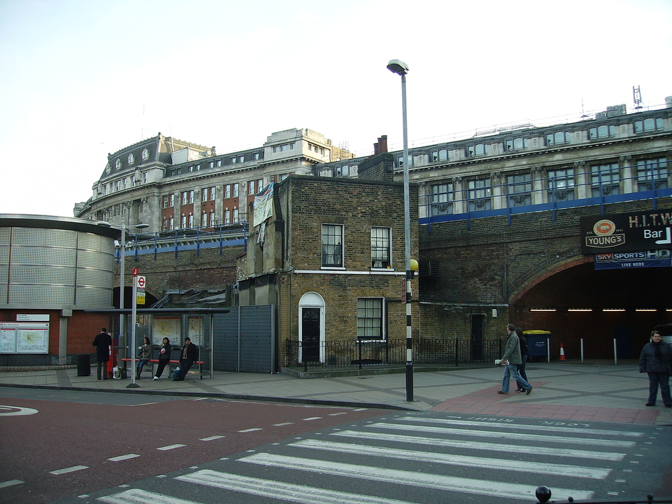
\includegraphics[width=\textwidth]{../imData/432/1.png}
		\caption{One image of the dataset we used for the puzzle with 432 pieces}
		\label{img:432}
	\end{subfigure}
	~
	\begin{subfigure}[b]{0.45\textwidth}
		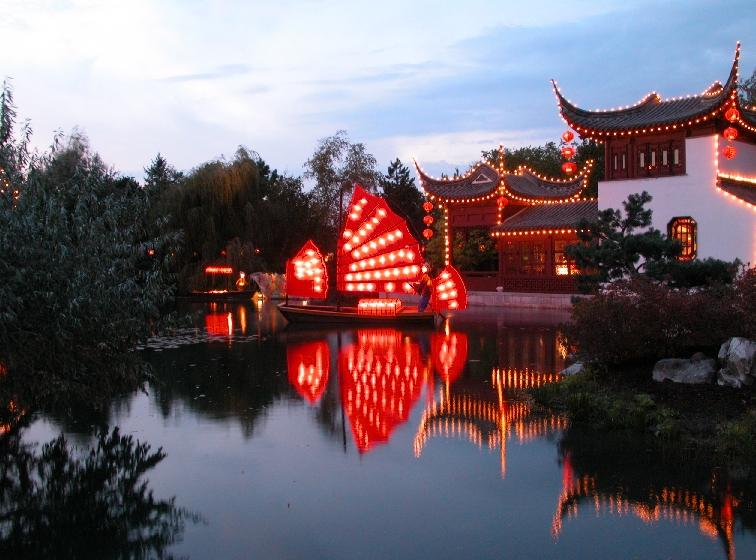
\includegraphics[width=\textwidth]{../imData/540/1.jpg}
		\caption{One image of the dataset we used for the puzzle with 504 pieces}
		\label{img:540}
	\end{subfigure}
	~
	\begin{subfigure}[b]{0.45\textwidth}
		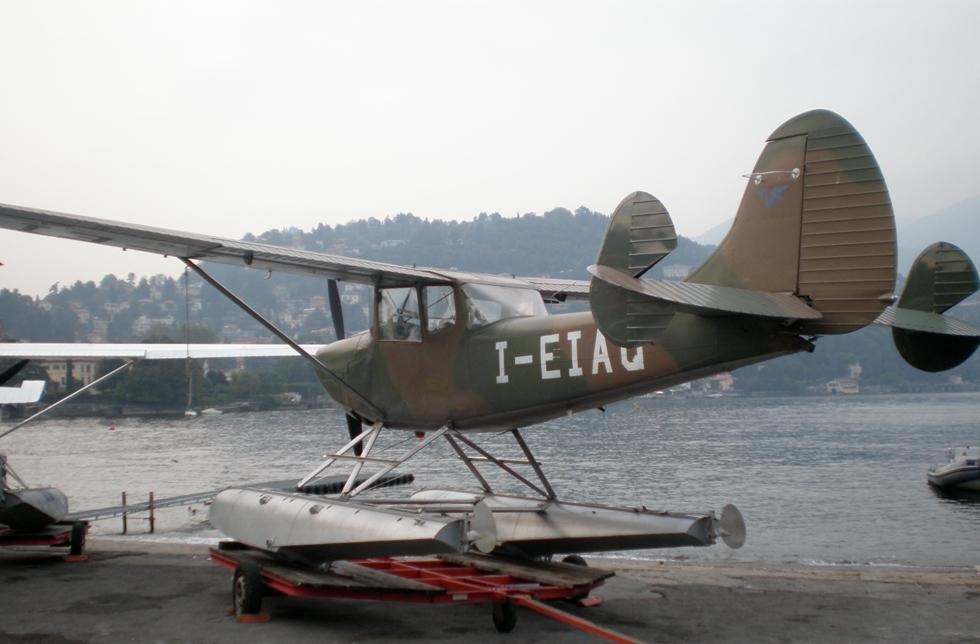
\includegraphics[width=\textwidth]{../imData/805/1.jpg}
		\caption{One image of the dataset we used for the puzzle with 805 pieces}
		\label{img:805}
	\end{subfigure}
	~
	\begin{subfigure}[b]{0.45\textwidth}
		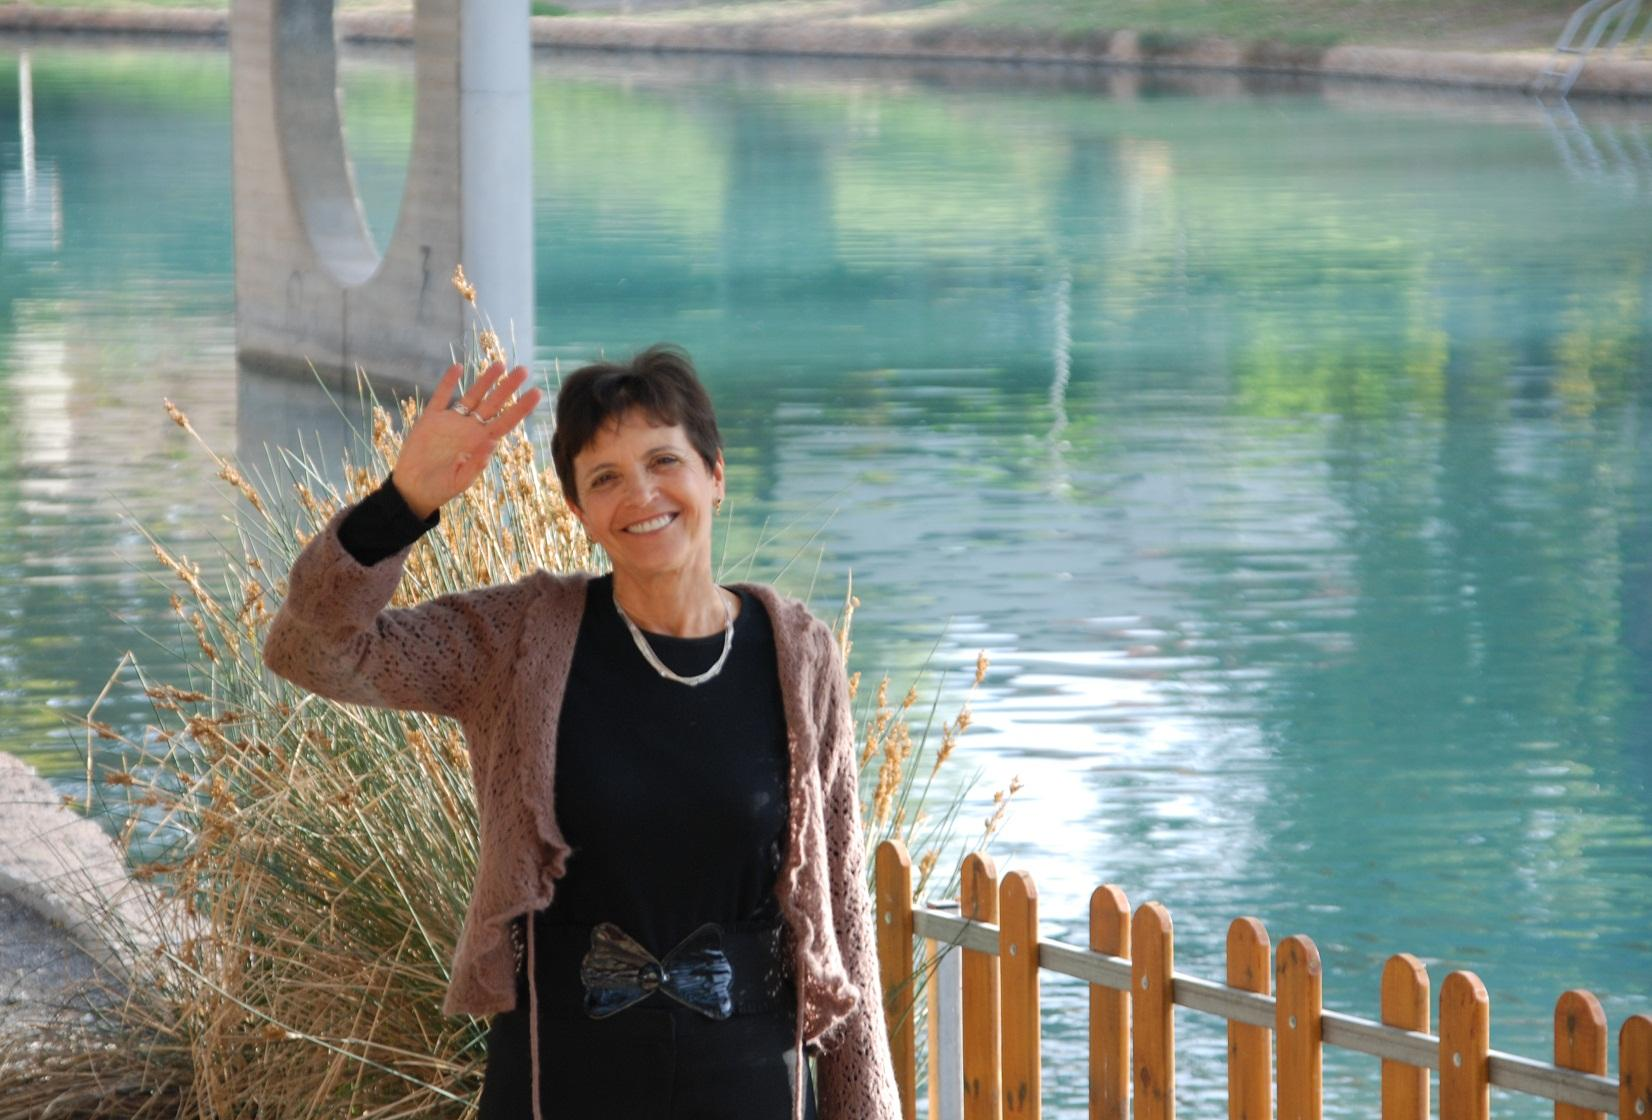
\includegraphics[width=\textwidth]{../imData/2360/1.jpg}
		\caption{One image of the dataset we used for the puzzle with 2360 pieces}
		\label{img:2360}
	\end{subfigure}

	\caption{A sample of all the datasets we used}
	\label{fig:database}
\end{figure}

To evaluate our results we used the direct measure, i.e. to check the absolute position of every piece in the image.


\chapter{Results}
\subsubsection{by Dominique Cheray}

\begin{table}[]
\centering
\caption{Comparison of our results to those of Paikin \& Tal \cite{Paikin2015}
  and those of Pomeranz et al.\cite{Pomeranz2011}}
\label{Results}
\begin{tabular}{@{}lllllll@{}}
\toprule
\multicolumn{1}{c ||}{}               & \multicolumn{3}{c||}{direct}                                                                                           & \multicolumn{3}{c}{perfect}                                                                                      \\ \midrule
\multicolumn{1}{l||}{\# of pieces} & \multicolumn{1}{c|}{Our}     & \multicolumn{1}{c|}{\cite{Paikin2015}} & \multicolumn{1}{c||}{\cite{Pomeranz2011}} & \multicolumn{1}{c|}{Our} & \multicolumn{1}{c|}{\cite{Paikin2015}} & \multicolumn{1}{c}{\cite{Pomeranz2011}} \\ \midrule \midrule
\multicolumn{1}{l||}{432}          & \multicolumn{1}{l|}{98.69\%} & \multicolumn{1}{l|}{96.16\%}             & \multicolumn{1}{l||}{90.95\%}               & \multicolumn{1}{l|}{11}  & \multicolumn{1}{l|}{13}                  & \multicolumn{1}{l}{13}                    \\ \midrule
\multicolumn{1}{l||}{540}          & \multicolumn{1}{l|}{88.21\%} & \multicolumn{1}{l|}{93.22\%}             & \multicolumn{1}{l||}{83.45\%}               & \multicolumn{1}{l|}{11}  & \multicolumn{1}{l|}{13}                  & \multicolumn{1}{l}{9}                     \\ \midrule
\multicolumn{1}{l||}{805}          & \multicolumn{1}{l|}{91.72\%} & \multicolumn{1}{l|}{92.47\%}             & \multicolumn{1}{l||}{80.25\%}               & \multicolumn{1}{l|}{7}   & \multicolumn{1}{l|}{9}                   & \multicolumn{1}{l}{7}                     \\ \midrule
\multicolumn{1}{l||}{2360}         & \multicolumn{1}{l|}{88.13\%} & \multicolumn{1}{l|}{94.01\%}             & \multicolumn{1}{l||}{33.4\%}                & \multicolumn{1}{l|}{0}   & \multicolumn{1}{l|}{1}                   & \multicolumn{1}{l}{1}                     \\ \midrule \midrule
\multicolumn{1}{l||}{Overall}  & \multicolumn{1}{l|}{91.69\%}    & \multicolumn{1}{l|}{93.97\%}              & \multicolumn{1}{l||}{72.01\%}  & \multicolumn{1}{l|}{29}  & \multicolumn{1}{l|}{36}                                       & \multicolumn{1}{l}{30}                                         \\ \bottomrule
\end{tabular}
\end{table}

As previously described, we evaluate our implementation of the algorithm with
the same image datasets as Paikin \& Tal \cite{Paikin2015}. These are three sets
of 20 pictures each, one for 432-piece puzzles, one for 540-piece puzzles and
one for 805-piece jigsaw puzzles. In addition, a record with three images for
puzzles with 2360 parts. Paikin and Tal evaluate their algorithm on additional
datasets for even larger puzzles (up to 22834 pieces). In the absence of the
necessary hardware needed for the computational effort to solve these puzzles we
are unable to evaluate our implementation with these datasets.

We compare our
results with those of Paikin \& Tal \cite{Paikin2015}, as well as with those of
Pomeranz et al. \cite{Pomeranz2011}, because the algorithm was inspired by their
work, and apply it to the classic puzzle problem, just like the works mentioned
above. This means the puzzle dimensions are known, there are no missing pieces
and no puzzles are mixed.

As a measure of accuracy, we use the common absolute measure, that is, the
proportion of pieces placed at their absolute correct position, and also report
the number of puzzles that have been perfectly reconstructed. Table
\ref{Results} shows the results, averaged for the respective datasets.

For the 432-pieces jigsaw puzzles, we can even outperform the results of Paikin \& Tal in
terms of direct measure by 2.5\%. Figure \ref{fig:success} shows an example of a
successful solved jigsaw puzzle of 432 pieces. But we can perfectly reconstruct only 11 images,
whereas Paikin \& Tal succeed at 13 images. Similarly, in comparison to Pomeranz et
al. We can clearly outperform their direct measure by almost 8\% however, they
can also perfectly reconstruct 13 images.

We can not quite reach the direct measure of Paikin \& Tal for the 540-pieces
jigsaw puzzles, we are 5 \% worse. And again we can perfectly reconstruct only 11
pictures, while they are doing so for 13 pictures. But we surpass Pomeranz et
al. both in terms of the direct measure, as well as the number of perfectly
reconstructed images. Our implementation of the algorithm makes the most
mistakes on images with large smooth regions or noisy images, as can be seen
exemplary in figure \ref{fig:fail}. On the left the original image on the right
the reconstructed image.

For the 805-pieces jigsaw puzzles, we achieve almost the same accuracy as Paikin
\& Tal when it comes to the direct measure and clearly outperform the results
of Pomeranz et al. Regarding the perfect reconstruction of images, we are two
images worse than Paikin \& Tal, but can perfectly reconstruct as many images as
Pomeranz et al.

Regarding the 2360-pieces jigsaw puzzles we are again not as good as Paikin \&
Tal, neither in terms of the direct measure nor in terms of the number of
perfectly reconstructed images. However, we clearly outperform the percentage of
correctly placed puzzle pieces by Pomerant et al. And both could perfectly
reconstruct only one of the three images.

Overall, our results on the number of correctly placed jigsaw puzzle pieces are
almost as good as those of Paikin \& Tal and much better than those of Pomeranz
et al. On the number of perfectly reconstructed images we achieve only one image
less than Pomeranz et al., but 7 less than Paikin \& Tal.
\begin{figure}
  \centering
  \begin{subfigure}{0.45\textwidth}
    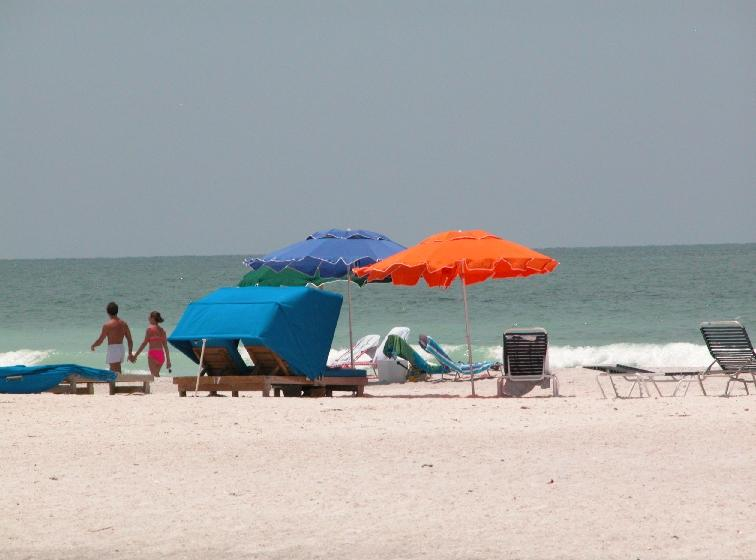
\includegraphics[width=\textwidth]{../imData/540/8.jpg}
		\caption{Original image}
		\label{img:540_8}
	\end{subfigure}
  \begin{subfigure}{0.45\textwidth}
  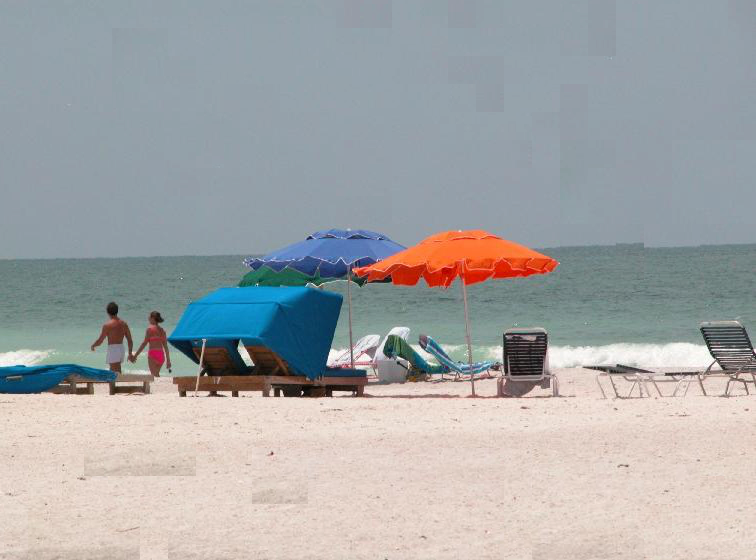
\includegraphics[width=\textwidth]{8_solved.png}
		\caption{Reconstructed image}
		\label{img:540_8_reconstructed}
	\end{subfigure}
  \caption{The algorithm may fail on images with large smooth regions or noisy images}
  \label{fig:fail}
\end{figure}

\begin{figure}
  \centering
  \begin{subfigure}{0.45\textwidth}
    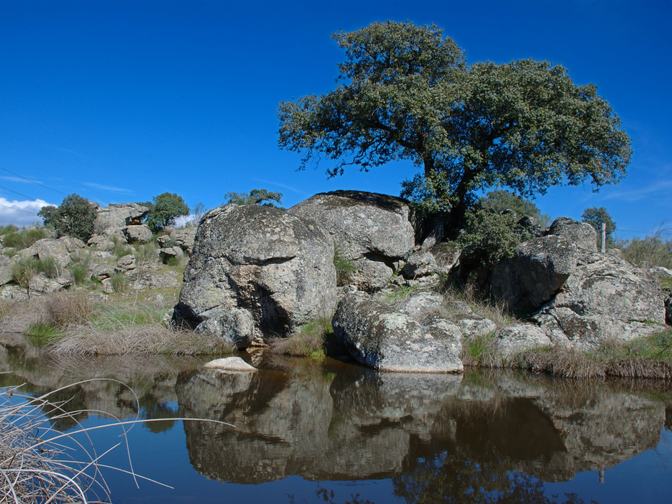
\includegraphics[width=\textwidth]{../imData/432/16.png}
		\caption{Original image}
		\label{img:432_8}
	\end{subfigure}
  \begin{subfigure}{0.45\textwidth}
  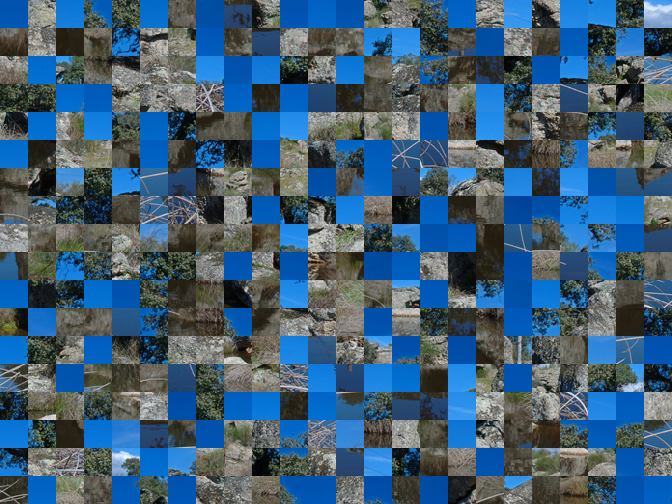
\includegraphics[width=\textwidth]{../results/432/16_shuffled.png}
		\caption{Shuffled input}
		\label{img:432:16_shuffled}
	\end{subfigure}
  \begin{subfigure}{0.45\textwidth}
  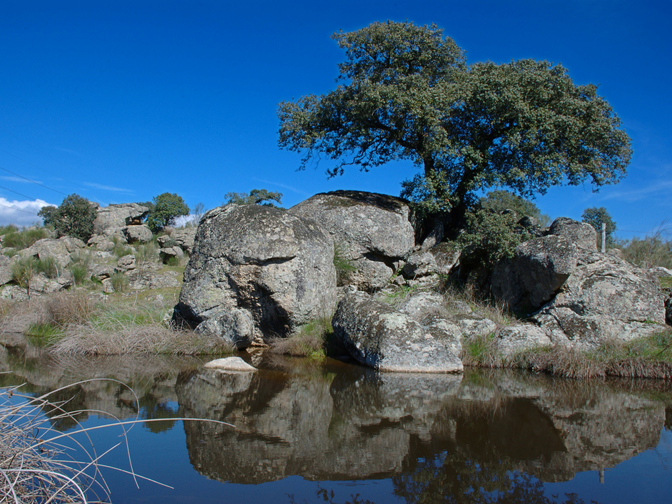
\includegraphics[width=\textwidth]{../results/432/16_solved.png}
		\caption{Reconstructed image}
		\label{img:432:16_solved}
	\end{subfigure}
  \caption{Example of a perfectly reconstructed image.}
  \label{fig:success}
\end{figure}

\chapter{Discussion}
\subsubsection*{by Manuel Krämer}

The purpose of this project was to build a puzzle solver based on \cite{Paikin2015} which produces comparable results. Within our limitations on time and resources we were able to reproduce and in some cases even improve the results from \cite{Paikin2015} and \cite{Pomeranz2011}.

As one can see in table \ref{Results} the absolute (direct) score of the 432 pieces puzzles is better than both results from the literature, although they have more perfectly solved puzzles. This means that they made more mistakes but only in a few images such that all others can be perfectly solved. A possible explanation of this behavior is that in \cite{Paikin2015} they didn't mention exactly how to place the pieces if the pool was empty (see chapter \ref{sec:algo}) so we tried several options like computing mutual compatibility to all pieces, all unplaced pieces, etc. As we tested our algorithm we obtained that most of the mistakes are made while placing the last few pieces and this would lead to a high direct score but a lot of not perfect results. This possible discrepancy in placing the last pieces could be investigated by implementing several options in the placer algorithm and comparing the final results to those of \cite{Paikin2015}.

Furthermore, the results of the puzzles with 540 pieces show similar relations as those with 432 pieces, despite the fact that the direct score is lower than the one from Paikin et al. This fact can be a consequence of the higher number of pieces; the most problems occur in the last part of the algorithm (placing the pieces if the pool was empty). If there are more pieces the probability to find best buddies gets smaller and the pool gets empty earlier with many unplaced pieces. This means that the problem that was described above occurs more often and the score decreases. In comparison to \cite{Pomeranz2011}, we achieve a better direct score and more perfect puzzles, what indicates that the overall approach as described in section \ref{sec:algo} (dissimilarity and mutual compatibility) is better than what Pomeranz et. al used.

The direct score and number of perfect puzzles of the 805 and 2360 pieces puzzles show similar results. As predicted above, the score gets much worse with a high number of pieces but is always better than the one from Pomeranz et al. The number of perfect puzzles for the 2360 pieces is 0 while \cite{Pomeranz2011} was able to achieve one. Here, the fact that the placer algorithm makes more 'late' mistakes with more pieces has so much impact on the results that there is no perfectly puzzled image although our direct score is more than twice as high as the one from \cite{Pomeranz2011}.

All in all, our project is able to verify the work from \cite{Paikin2015}. Since their description of the algorithm is more like a rough outline there are many points where we could do minor changes to improve the results until they are equal to those from \cite{Paikin2015}. Moreover one could implement another measure of accuracy, e.g. the neighbor measure as used in \cite{Paikin2015}. We would expect that this measure leads to equal results as those from Paikin et al. because the direct measure (and number of perfect puzzles) is not good for minor mistakes that e.g. shift the pieces: This could lead to a direct measure of 0 although almost all pieces found their correct neighbor. 


\nocite{*}

\bibliography{literature}

\end{document}          
         
